\documentclass[a4paper]{scrreprt}
 
\usepackage[german]{babel}
\usepackage[utf8]{inputenc}
\usepackage[T1]{fontenc}
\usepackage{ae}
\usepackage[bookmarks,bookmarksnumbered]{hyperref}
\usepackage{graphicx}
\usepackage{floatflt}
\usepackage{enumitem}
\usepackage{pifont}
\setlength{\parindent}{0pt}
 
\begin{document}
 
\title{Entwicklerdokumentation}
\subtitle{ILIAS Review Plugin}
\publishers{Version: 1.0, Status: in Arbeit}
\author{SWT-Gruppe 04\\ \\Auftraggeber: Thordis Kombrink\\Weitere: Dr Birgit Demuth, Professor Wollersheim\\Tutor: Andy Püschel}
\maketitle


\tableofcontents
\chapter{Einführungen und Ziele}
\section{Aufgabenstellung}
Aufgabe ist es ein Plugin für das freie, internetbasierte Lernsystem ILIAS\footnote{\url{http://www.ilias.de/docu/ilias.php?baseClass=ilrepositorygui&reloadpublic=1&cmd=frameset&ref_id=1}} zu programmieren, um es um eine Review-Möglichkeit der erstellten Fragen zu erweitern. 
\section{Qualitätsziele}
\begin{tabular}{|c|c|c|c|c|}\hline
Anforderung & Sehr wichtig & Wichtig & Normal & Irrelevant \\\hline
Funktionalität &\ding{51}&&&\\\hline
Benutzerfreundlichkeit &\ding{51}&&&\\\hline
Erweiterbarkeit &&\ding{51}&&\\\hline
Zuverlässigkeit &&\ding{51}&&\\\hline
Korrektheit &&\ding{51}&&\\\hline
Sicherheit &&&\ding{51}&\\\hline        
Effizienz &&&\ding{51}&\\\hline
Portierbarkeit &&&&\ding{51}\\\hline
\end{tabular}
\section{Stakeholder}
\begin{tabular}{|p{3.5cm}|p{2.3cm}|p{3cm}|p{4cm}|}\hline
Name & Rolle & Beschreibung & Intention \\\hline
Thordis Kombrink & Kundin & Mitarbeiterin an der Fakultät Informatik, zugehörig zum Lehrstuhl Systems-Engineering & -möchte in ihrer Arbeitsgruppe Ilias nutzen, um Klausuren zu erstellen, mit gereviewten Fragen\\\hline
Dr. Birgit Demuth & Interessentin & Arbeitet am Lehrstuhl Softwaretechnologie & -Interesse an der Umsetzung, um Ilias unter Umständen an der Fakultät einzusetzen\\\hline
Prof. Dr. Heinz-Werner Wollersheim & Fachlicher Ansprechpartner & Professor aus Leipzig der sich mit dem Thema (Fragen für Klausuren reviewen) auseinandersetzt & -würde gerne effektiver mit Ilias in seiner Arbeitsgruppe arbeiten, es fehlt aber die Reviewmöglichkeit, die wir erstellen\\\hline
\end{tabular}
\chapter{Randbedingungen}
\section{Konventionen} 
Das Plugin muss die ILIAS-Version 4.4.5, die MySQL Version 5.0.11 und die PHP-Version 5.5.11 unterstützen.\\
Es gelten die im 'Ilias-Developement-Guide'\footnote{\url{http://www.ilias.de/docu/goto.php?target=lm_42&client_id=docu} (29.10.14)} und in den 'Ilias Usability and Accessibility Guidelines'\footnote{\url{http://www.ilias.de/docu/goto_docu_lm_459.html} (29.10.14)} festgesetzten Konventionen.
\chapter{Kontextabgrenzung}
\section{Fachlicher Kontext}
Für die Reviews sind mehrere Plugins notwendig. Zum einen soll ein Plugin entwickelt werden, das die Verwaltung von Reviews ermöglicht, zum anderen müssen Plugins für Reviewbare Fragen erstellt werden. Das Review-Plugin stellt die Benutzeroberflächen bereit und beinhaltet die Review-Datenbank.\\
Als Beispiel für ein Plugin einer reviewbaren Frage wurde das Plugin der reviewbaren Multiple-Choice-Frage gewählt.\\
Für die Plugins werden verschiedene Plugin-Slots verwendet. Ilias stellt eine Schnittstelle für neue Fragen bereit. Das Verwaltungs-Plugin soll als Repository-Plugin erstellt werden.\\ 
(siehe nächste Seite)\\

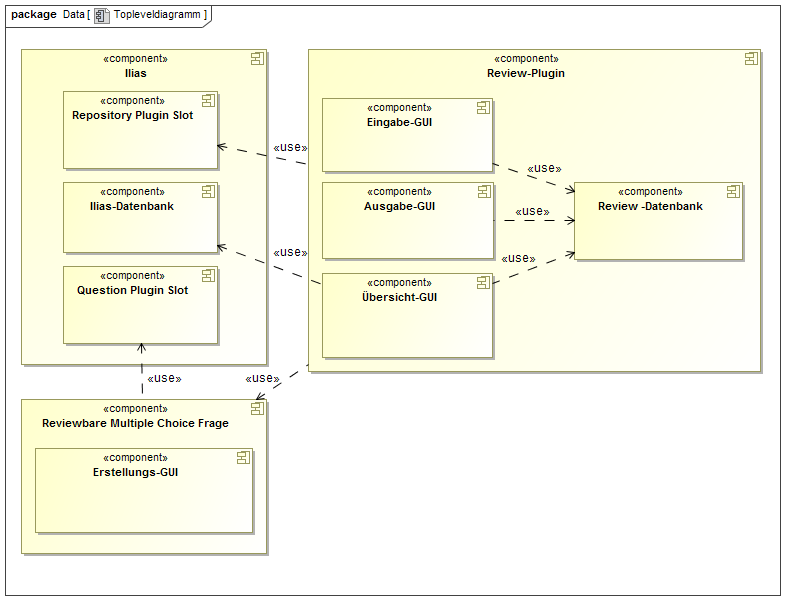
\includegraphics[width=1.0\textwidth]{Component_Diagram__Topleveldiagramm.png}
\label{Toplevel-Architektur}
\section{Technischer- oder Verteilungskontext}
\section{Externe Schnittstellen}
\texttt{Review}\\

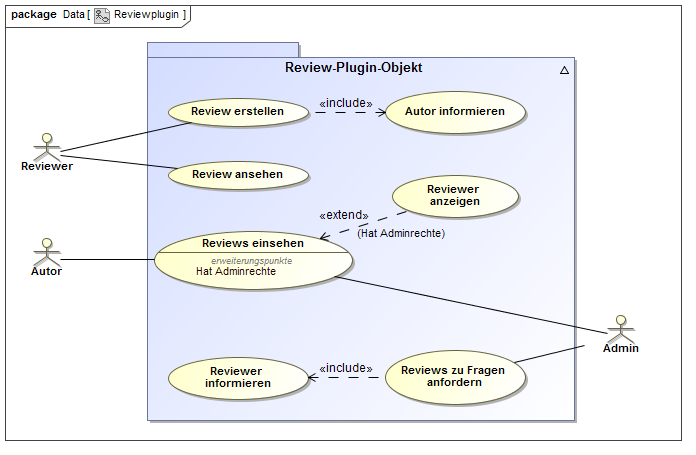
\includegraphics[width=1.0\textwidth]{Use_Case_Diagram__Reviewplugin.png}
\label{Review}

\begin{tabular}{|p{0.5cm}|p{3cm}|p{0.5cm}|p{4cm}|p{4.5cm}|}\hline
Nr. & Anwendungsfall & Nr. & Anfrage & Antwort\\\hline
1.0 & Ein Administrator fordert Reviews & 1.1 & Es ist noch kein Review vorhanden & Die vom Administrator zur Frage zugeordneten Reviewer werden ermittelt und unbearbeitete Reviews erstellt. Die Reviewer werden darüber informiert, dass sie ein Review zu schreiben haben.\\\hline
&&1.2 & Es sind bereits Reviews zu der Frage vorhanden. & Die bereits vorhandenen Reviews werden auf unbearbeitet gesetzt. Die Reviewer werden darüber informiert.\\\hline
2.0 & Reviewer erstellt ein Review & 2.1 & Der Reviewer füllt alle Felder vollständig aus. & Das Review wird auf bearbeitet gesetzt und in der Datenbank gespeichert. Zudem wird vermerkt das wievielte Review der Reviewer gegeben hat.\\\hline
&&2.2 & Der Reviewer vergisst, Felder auszufüllen. & Der Reviewer erhält eine Meldung, dass er vergessen hat manche Felder auszufüllen. \\\hline
3.0 & Reviewer betrachtet Reviews & 3.1 & Der Reviewer versucht Reviews einzusehen & Der Reviewer erhält eine Übersicht nur über das von ihm gegebene Review. \\\hline
4.0 & Autor betrachtet Reviews & 4.1 & Es sind Reviews vorhanden & Der Autor erhält eine Übersicht über alle bereits gegebenen Reviews, allerdings kann er die Informationen zu den Reviewern nicht einsehen. \\\hline
5.0 & Administrator betrachtet Reviews & 5.1 & Es sind Reviews vorhanden & Der Administrator erhält eine vollständige Übersicht über die gegebenen Reviews. \\\hline
\end{tabular}
 
\newpage
\texttt{Fragepool}\\

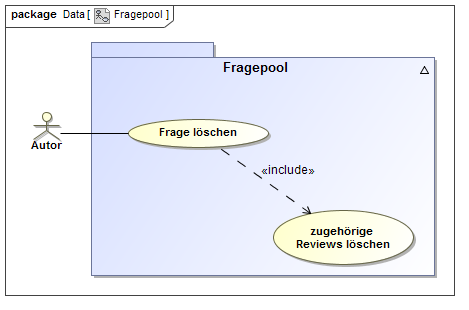
\includegraphics[width=1.0\textwidth]{Use_Case_Diagram__Fragepool.png}
\label{Fragepool bearbeiten}

\begin{tabular}{|p{0.5cm}|p{3cm}|p{0.5cm}|p{4cm}|p{4.5cm}|}\hline
Nr. & Anwendungsfall & Nr. & Anfrage & Antwort\\\hline
1.0 & Autor löscht eine Frage & 1.1 & Reviews vorhanden & Zugehörige Reviews werden gelöscht\\\hline
\end{tabular}


\chapter{Lösungsstrategie und Entwurfsentscheidungen}
\section{Datenbankstruktur}

Folgende Datenbanken werden durch die Plugins erstellt:\\
\begin{tabular} {| l | l |}\hline
Name & Beschreibung \\\hline
qpl\textunderscore rev\textunderscore qst & beinhaltet die Taxonomie und die Wissensdimension alles Fragen \\\hline
rep\textunderscore robj\textunderscore xrev\textunderscore revobj & Standardtabelle für Review-Plugin-Objekte, speichert Gruppen-Id \\\hline
rep\textunderscore robj\textunderscore xrev\textunderscore quest & speichert Review-spezifische Frage-Informationen \\\hline
rep\textunderscore robj\textunderscore xrev\textunderscore revi & speichert alle Review-Daten \\\hline
rep\textunderscore robj\textunderscore xrev\textunderscore taxon & beinhaltet alle Taxonomie-Stufen \\\hline
rep\textunderscore robj\textunderscore xrev\textunderscore knowd & beinhaltet alle Knowledge-Dimensionen \\\hline
rep\textunderscore robj\textunderscore xrev\textunderscore rate & beinhaltet Fragen-Bewertungsmöglichkeiten \\\hline
rep\textunderscore robj\textunderscore xrev\textunderscore eval & beinhaltet Bewertungsmöglichkeiten für einzelne Aspekte der Fragen \\\hline
rep\textunderscore robj\textunderscore xrev\textunderscore expert & beinhaltet alle möglichen Expertisen für Reviewern \\\hline
\end{tabular}

\section{Reviewbare Frage-Plugin}
Im Rahmen der Analyse-Phase haben wir festgestellt, dass ein Plugin nicht ausreichend ist, da die bisher vorhandenen Fragen nicht den Kriterien unseres Vorhabens entsprechen. Ein Musskriterium war, dass die Taxonomie-Einordnung hinzugefügt wird, diese ist in Ilias aber nicht so vorhanden, wie wir sie benötigten, aus diesem Grund haben wir den neuen Fragentyp erstellt.\\
Die Reviewbare Frage unterscheidet sich nur wenig von den bereits in Ilias vorhandenen Fragen, es wurde lediglich bei der Fragenstellung ein neuer Absatz hinzugefügt, zum Angeben der Taxonomie-Einordnung. \\
\subsection{Ordnerstruktur}
Die Ordnerstruktur richtet sich nach den Ilias-Konventionen\footnote{\url{http://www.ilias.de/docu/ilias.php?ref_id=42&obj_id=27029&cmd=layout&cmdClass=illmpresentationgui&cmdNode=ih&baseClass=ilLMPresentationGUI&obj_id=64260}} für das "Test Question Plugin". Die Datei plugin.php definitert die ID des Plugins (revmc) und die kompatiblen ILIAS-Versionen (4.4.xx), außerdem hält sie die aktuelle Version des Review-Plugins fest\\
Im Ordner "classes" befinden sich die "...Plugin"- und "...Feedback"-Klassen, welche von Ilias' Multiple-Choice-Frage übernommen wurden. In den Unterordnern "import" und "export" befinden sich die PHP-Dateien, welche für die Auslagerung und Wiedereinbindung von Fragen zuständig sind. 
In der GUI-Datei wurde ein Großteil der Elemente übernommen. Um die Taxonomien anzugeben, haben wir uns für Aufklappmenüs entschieden(in Ilias ilSelectInputGUI()), da bei diesen aus mehreren Auswahlmöglichkeiten genau eine ausgewählt wird. Davon nutzen wir zwei zum Angeben der Wissensdimension und der Taxonomie.\\
Die GUI speichert und läd auch die Daten aus der Datenbank, in der Datenbank werden die Eigenschaften als Integerwerte abgespeichert, welche über Funktionen in die entsprechenden Taxonomie-Werte umgewandelt werden.\\
\\
Im Ordner "lang" befinden sich die entsprechenden Language Dateien für Deutsch und Englisch, in denen den Variablen die Ausdrücke zugeordnet werden.\\
Der Ordner "sql" beinhält die Datenbank-Verwaltungs-Datei dbupdate.php, in welcher neue Tabellen anlegt werden.\\
Im Ordner "templates" befinden sich die Template Dateien, die den Content von der Multiple Choice Frage übernehmen.

\section{Review-Plugin}
\subsection{Allgemein}
Die Struktur des Review-Plugins richtet sich nach der Vorgabe für Repository Object Plugins, weil es gegen diese Plugin-Schnittstelle geschrieben wurde. Die Datei plugin.php definitert die ID des Plugins (xrev) und die kompatiblen ILIAS-Versionen (4.4.xx), außerdem hält sie die aktuelle Version des Review-Plugins fest\\
Im Unterordner classes befinden sich die Klassen, die ILIAS von einem Repository Object Plugin fordert. Diese müssen dazu jeweils eine plugintypspezifische Oberklasse, die der Funktionalität der betreffenden Klasse entspricht, erweitern. Durch dieses Prinzip können wir sehr viele ILIAS-Komponenten wiederverwenden und erreichen automatisch eine Trennung von Anwendungslogik und Benutzeroberfläche. Die Anwendungslogik steht in der Klasse ilObjReview, die von ilObjectPlugin erbt, und ilObjReviewGUI, das von ilObjectPluginGUI erbt, ist der GUI-Controller (auf beide Klassen wird unten detailliert eingegangen). Die Klasse ilObjReviewAccess, die Zugriffe überprüft, erweitert die ihr zugehörige Oberklasse ilObjectPluginAccess und implementiert als neue Funktionalität im wesentlichen die Überprüfung, ob ein Nutzer tatsächlich berechtigt ist, auf ein von ihm angefordertes Objekt zuzugreifen (siehe dazu den Gliederungspunkt Sicherheit). Um Review-Objekte in der Gruppenübersicht anzeigen zu können, ist die Klasse ilObjReviewListGUI nötig, die von ilObjectPluginListGUI erbt. DIe Grundklasse ilReviewPlugin, die von ilRepositoryObjectPlugin erbt, muss laut Spezifikation nur den Namen des Plugins zurück geben und wurde entsprechend gering gehalten.\\
Der Unterordner lang enthält die Sprachdateien in der Form ilias\textunderscore[Sprachkürzel].lang, in denen die Texte der Benutzeroberfläche ausgelagert sind, um den Anforderungen an die Internationalisierung des Plugins gerecht zu werden (siehe dazu den Gliederungspunkt Internationalisierung).\\
Im Unterverzeichnis sql befindet sich die Datei dbupdate.php, ein Datenbank-Updateskript, das bei jeder neuen Version des Plugins von ILIAS ausgeführt wird. Es beinhaltet das Anlegen aller Tabellen des Plugins in der ILIAS-Datenbank sowie die Füllung derjenigen Tabellen, die Enumerationen darstellen, mit ihren Einträgen.\\
Der Unterordner Templates enthält die Ordner images und default. In images sind die Icons des Plugins abgelegt, während default Templates für die eigenen GUI-Klassen des Plugins erhält. Jene befinden sich im Verzeichnis classes/GUI und werden unten detailliert erläutert.
\subsection{Besonderheiten der Anwendungslogik - ilObjReview}
Diese Klasse repräsentiert ein Review-Objekt, das zusätzlich zu den Attributen seiner Oberklasse noch über eine group\textunderscore id, die ID der Gruppe in der das Review-Objekt angelegt wurde, verfügt. Das von ilObjectPlugin geerbte Attribut obj\textunderscore id wird verwendet, um die Daten verschiedener Review-Objekte, die in einer ILIAS-Installation existieren können, in der Datenbank auseinanderhalten zu können.\\
Die Klasse ilObjReview.php überschreibt die Methoden doCreate, doRead, doUpdate, doDelete und doClone ihrer Oberklasse, die zur Aktualisierung der Datanbank bei der Erstellung, beim Öffnen, beim Bearbeiten, beim Löschen bzw. beim Klonen eines Review-Objekts aufgerufen werden. Die Methode doCreate liest dazu die Gruppen-ID, die bei der Erstellung eines neuen Repository-Objekts in einer Gruppe von ILIAS als Parameter angehängt wird, aus. Die Methode doRead, die jedes Mal, wenn ein Nutzer auf ein Review-Objekt zugreift, aufgerufen wird, ruft zusätzlich die private Methode syncQuestionDB auf, die die Fragendatenbank von ILIAS an die des Review-Objekts angleicht. Die Methode doDelete scheint von ILIAS nicht aufgerufen zu werden, weshalb auf eine Implementierung verzichtet wurde.\\
Die Funktionsweise von syncQuestionDB ist die Folgende: zunächst werden alle Fragen aus den Fragepools der Gruppe, in der das Review-Objekt angelegt wurde, und alle Fragen aus der Fragendatenbank des Review-Objektes geladen jeweils in einer Datenstruktur gespeichert. Fragen, die in beiden vorkommen, werden auf ihren Timestamp überprüft; hat die Frage aus dem Fragenpool einen neueren, ist sie seit dem letzten Aufruf des Review-Objekts bearbeitet worden. Dementsprechend wird ihr Zustand auf 0 gesetzt und von den dieser Frage zugeteilten Reviewern werden neue Reviews angefordert (Aufrufe von \$ilDB->update), außerdem werden die Reviewer darüber benachrigtigt (Aufruf von notifyReviewersAboutChange). Ist eine Frage nur in einem Fragepool enthalten, dann wurde sie neu erstellt und wird der Datenbank hinzugefügt (Aufruf von \$ilDB->insert) und die Administratoren werden drüber informiert (Aufruf von notifyAdminsAboutNewQuestion). Ist eine Frage nur in der Datenbank des Review-Objekts vorhanden, dann wurde sie im Fragepool gelöscht und wird nun automatisch mitsamt der zur ihr gehörenden Reviews aus der Datenbank des Review-Objekts entfernt (Aufruf von \$iDB->manipulateF) und die vormaligen Reviewer weden informiert (notifyReviewersAboutDeletion).\\
Der Großteil der weiteren Methoden sind Datenbankabfragen, die Reviews, Fragen oder andere Datensätze abrufenund als assoziative Arrays zurückgeben. Diese Methoden sind deshalb notwendig, da das Plugin mehrere Anwendungsfälle abdeckt, für welche Daten unter unterschiedlichen Kriterien ausgewählt und formatiert werden müssen. Von besonderer Bedeutung sind die Methoden allocateReviews und storeReviewById. Erstere legt, nachdem der Administrator einer Frage Reviewer zugeordnet hat, leere Review-Datensätze in der Datenbank an und letztere aktualisiert einen solchen Datensatz, nachdem ein Nutzer ein Review-Eingabeformular ausgefüllt hat, um die eingegebenen Daten. Die Methode finishQuestion aktualisiert den Zustand von Fragen, die akzeptiert werden, sodass sie von den anderen Funktionen des Plugins nicht mehr berücksichtigt werden.\\
Die Methoden taxonomy, knowledgeDimension, expertise, rating und evaluation laden die jeweilige Enumeration aus der Datenkbank, damit sie später in Aufklappmenüs verwendet werden können.\\
Wann immer ein Fall eintritt, der eine Benachrichtigung erfordert, wird direkt die zur Nachricht gehörige notify...-Methode dieser Klasse aufgerufen. Sie ermittelt die Empfänger der Nachricht und übergibt diese gemeinsam mit der eigentlichen Benachrichtigung der privaten performNotification-Methode, die die eigentliche Systemnachricht erstellt und abschickt. Dabei steht der eigentliche Text in den Sprachdateien (siehe oben), während die Methoden nur Keys für diesen Text übergeben.
\subsection{Besonderheiten des GUI-Controllers - ilObjReviewGUI}
Die Controller-Klasse für die GUI erbt fast alle Funktionalitäten von ilObjectPluginGUI, darunter auch eine Referenz auf die Anwendungsklasse ilObjReview. Die von anderen, ILIAS-internen Controllern aufgerufenen Methoden performCommand und setTabs führen einen Befehl aus bzw. zeigen die Tabs, in die die Benutzeroberfläche unterteilt ist, an. Dabei überprüfen sie jeweils, ob der Nutzer die erforderlichen Rechte hat.\\
Durch getAfterCreationCmd und getStandardCmd bestimmt, wird bei Aufruf des Review-Objektes zunächst der Befehl showContent ausgeführt, der eine Übersicht über Fragen und Reviews eines Nutzers erzeugt. Diese sind jeweils in externe GUI-Klassen ausgelagert, die unten erläutert werden.\\
Bei Klicks auf die Tabelleneinträge oder die Tabs ermittelt ILIAS anhand der gespeicherten Link-Variablen den nächsten auszuführenden Befehl, der dann das Eingabeformular für den Nutzer bereitstellt. Das können die vier Befehle inputReview, editProperties, allocateReviews oder finishQuestions sein, die zunächst die GUI für das Review-Eingabeformular, Bearbeitung der Eigenschaften des Review-Objekts, Zuordnung von Reviewern zu Fragen bzw. Akzeptieren von gereviewten Fragen erstellen. Dabei verwenden sie die eigene GUI-Klasse ilReviewInputGUI bzw. die privaten Methoden initPropertiesForm, initReviewAllocForm und initQuestionFinishForm, die ihrerseits wieder auf eigene GUI-Klassen zurückgreifen. Sie setzen die Ziele der Absenden-Buttons auf die zugehörigen Befehle saveReview, updateProperties, saveAllocateReviews bzw. saveFinishQuestions, die die eingegebenen Daten überprüfen und bei Erfolg mithilfe der entsprechenden Methode von ilObjReview in der Datenbank speichern.\\
Ein weiterer Befehl dieses GUI-Controllers ist showReviews, der alle Reviews, die zu einer Frage gehören, mithilfe von ilReviewOutputGUI ausgibt.
\subsection{Besonderheiten der eigenen GUI-Klassen}
Im Unterverzeichnis classes/GUI wurde eine Reihe eigener GUI-Klassen in Form von Tabellen und Eingabeelementen erstellt, da die ILIAS-Komponenten nicht in allen Fällen genügt haben. Dabei nutzen sie die Template-Engine von ILIAS, um ihre visuelle Darstellung zu beschreiben, indem sie die HTML-Templates aus dem Ordner templates/default und die Stylesheets aus dem Verzeichnis templates/default/CSS einbinden.\\
ilAspectHeadGUI und ilAspectSelectGUI ermöglichen es, mehrere Textfelder (ilNonEditableValueGUI) bzw. Aufklappmenüs (ilSelectInputGUI) nebeneinander auf einer Zeile darzustellen. Zu diesem Zweck erweitern sie ilCustomInputGUI, in der die Grundfunktionalitäten für eigene GUI-Klassen bereits implementiert sind.\\
ilCheckMatrixRowGUI funktioniert ähnlich, aber für Checkboxen, die für die Reviewer-Zuordnung in einer Matrix angeordnet werden, wobei vertikal die Fragen und horizontal die Gruppenmitglieder angeordnet werden. Für jede Frage existiert also eine Instanz von ilCheckMatrixRowGUI, die für jedes Gruppenmitglied eine Checbox innehat. Die Postvariablen für die einzelnen Checkboxen werden im Konstruktor dynamisch erzeugt und können mittels getPostVars vom GUI-Controller abgerufen werden.\\
ilQuestionFinishTableGUI, ilQuestionTableGUI und ilReviewTableGUI erzeugen jeweils eine tabellanartige Ansicht der zu beendenden Fragen, der Fragen eines Nutzers bzw. der Reviews eines Nutzers anhand der bei der Erstellung übergebenen Datensätze. Dazu erweitern sie die ILIAS-Klasse ilTable2GUI.\\
ilQuestionOverviewGUI erzeugt lediglich eine Ansicht einer Frage, mit der der Nutzer nicht interagieren kann. Desahlb verwendet sie ausschließlich ein Template und erweitert keine ILIAS-Komponente.\\
ilReviewInputGUI erzeugt das Review-Eingabeformular. Sie erweitert dazu ilPropertyFormGUI, die Standard-Formularklasse vonn ILIAS und erzeugt sowohl GUI-Elemente, die von ILIAS stammen, als auch eigene. Dazu müssen ihr der betreffende Reviewdatensatz und die Taxonomie der gereviewten Frage übergeben werden, außerdem erwartet sie die vom Plugin definierten Enumerationen als Parameter. Nach Aufruf der Methode setReadOnly können die GUI-Elemente von ilObjReviewGUI deaktiviert werden, sodass diese Klasse für die Review-Ausgabe wiederverwendet werden kann. Die Methode checkInput der Oberklasse wurde überschrieben, um bei den Aufklappmenüs sicherszustellen, dass ein anderer Wert als der default-Wert ausgewählt wurde.\\
Die Review-Ausgabeklasse ilReviewOutputGUI erweitert ebenfalls ilTable2GUI, um Review-Eingabeformulare in einer Tabelle darzustellen. Diese werden durch Instanzen von ilReviewInputGUI gebildet, die aufgrund eines Aufrufs von setReadOnly nicht mehr bearbeitet werden können. Diese Klasse erwartet zur Konstruktion ein Array von Reviews und ansonsten die gleichen Daten wie ilReviewInputGUI. Zum Erstellen der Ausgabe kann sie dadurch einfach über die gegebenen Reviews iterieren und für jedes von ihnen mit den gegebenen Daten ein Eingabeformular erstellen.
\chapter{Bausteinsicht}
\chapter{Laufzeitsicht}
\chapter{Konzepte}
\section{Fachliche Strukturen und Modelle}
\texttt{Analyseklassendiagramm}\\
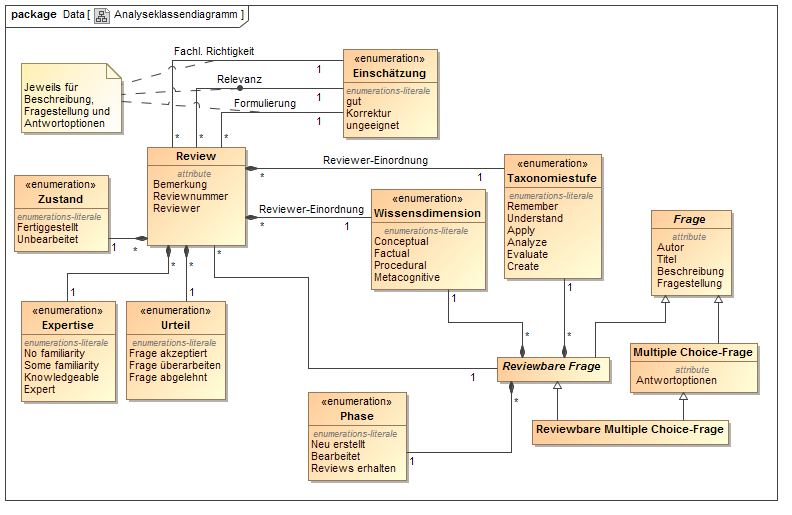
\includegraphics[width=1.0\textwidth]{Class_Diagram__Analyseklassendiagramm.png}
\label{Analyseklassendiagramm}

\newpage
\texttt{Review anfordern}\\
Nachdem der Autor eine Frage erstellt hat, kann er ein Review anfordern. Dadurch werden Reviewer bestimmt, welche vom Review-Plugin informiert werden, dass ein Review abzugeben ist.\\

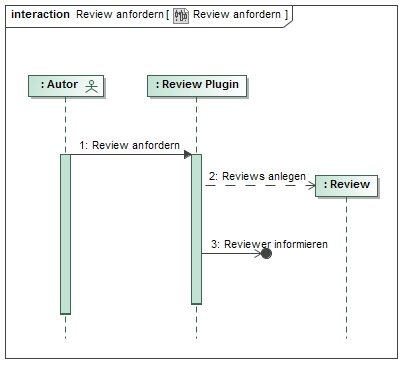
\includegraphics[width=1.0\textwidth]{Sequence_Diagram__Review_anfordern__Review_anfordern.png}
\label{Review anfordern}

\newpage
\texttt{Review abschließen}\\
Wenn ein Reviewer sein Review abgeschlossen hat, werden die Review-Daten formatiert und abgespeichert. Im Anschluss wird der Autor informiert, dass ein neues Review vorhanden ist.\\

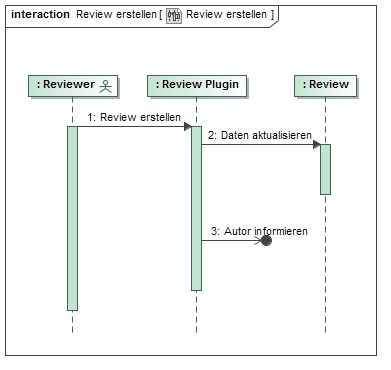
\includegraphics[width=1.0\textwidth]{Sequence_Diagram__Review_erstellen__Review_erstellen.png}
\label{Review beenden}
\section{Persistenz}
Um Persistenz zu ermöglichen, nutzen wir die mySQL-Datenbankverwaltung, wie sie in Ilias implementiert ist.
\section{Benutzungsoberfläche}
\centering
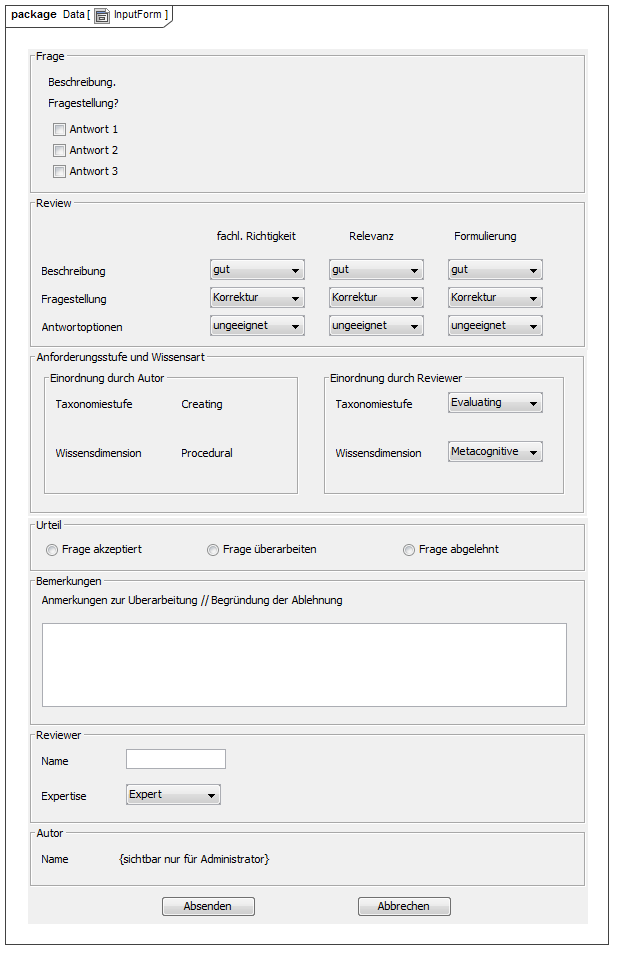
\includegraphics[width=0.88\textwidth]{User_Interface_Modeling_Diagram__InputForm.png}
\label{Grafische Benutzeroberfläche}\newpage
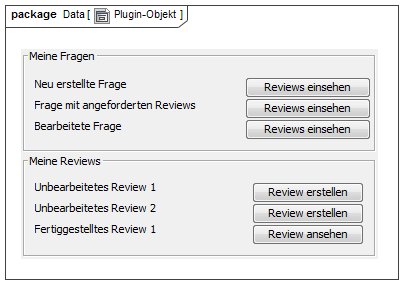
\includegraphics[width=0.99\textwidth]{User_Interface_Modeling_Diagram__Plugin-Objekt.png}
\label{Grafische Benutzeroberfläche Autor}
\\
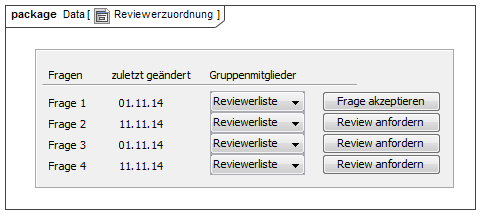
\includegraphics[width=0.7\textwidth]{User_Interface_Modeling_Diagram__Reviewerzuordnung.png}
\label{Grafische Benutzeroberfläche Autor}
\section{Ergonomie}
\flushleft
{Peter}
\section{Transaktionsbehandlung}
\section{Sessionbehandlung}
\section{Sicherheit}
Da das Plugin in das ILIAS-System eingebettet ist und die bereits erstellten ILIAS-Komponenten wiederverwendet, gelten dieselben Sicherheitsstandards. Nutzereingaben und Datenbankabfragen werden daher durch ILIAS-Komponenten überprüft und das Plugin passt sich nahtlos in die Benutzerverwaltung von ILIAS und ihr Rechtesystem ein. Eine mögliche Sicherheitslücke in ILIAS ist das Anhängen von IDs als GET-Parameter an die Adresse. Um diese zu schließen, haben wir vor jede Anzeige eines Formulars eine Validierung geschaltet, die überprüft, ob der Nutzer tatsächlich auf das Objekt, welches als GET-Parameter angehängt ist, zugreifen darf. 
\section{Kommunikation und Integration mit anderen IT-Systemen}
!!!!!max, lassen sich aus anderen systemen fragen einbinden? wenn ja, schreiben wir das hier hin! :)!!!!
\section{Verteilung}
\section{Plausibilisierung und Validierung}
Wir greifen auf Nutzereingaben mittels der bereits implementieren GUI-Komponenten von ILIAS zu. Diese überprüfen die Nutzereingabe intern und somit transparent für unser Plugin. Die Benutzerauthentifizierung ist ebenfalls von ILIAS gedeckt, lediglich die unter „Sicherheit“ genannte Möglichkeit, dass der Benutzer bei Aufruf eines Formulars den ID-Parameter in der Adressleiste ändert und somit unberechtigt auf Daten zugreift, musste von uns ausgeschlossen werden.
\section{Ausnahme-/Fehlerbehandlung}
\section{Logging, Protokollierung, Tracing}
\section{Konfigurierbarkeit}
\section{Internationalisierung}
Das Plugin enthält ein Englisches und ein Deutsches Sprachpaket. Weitere Sprachen lassen sich über die Ilias-Konforme Einbettung\footnote{\url{http://www.ilias.de/docu/ilias.php?ref_id=37&obj_id=8478&from_page=133&cmd=layout&cmdClass=illmpresentationgui&cmdNode=ih&baseClass=ilLMPresentationGUI&obj_id=128}} 
 
\section{Testbarkeit}
Peter
\section{Buildmanagement}
Für das Plugin wurden PHP-Dateien geschrieben, die beim Starten von Ilias in dessen Hauptdateien eingebunden werden.\\
Es wurden 2 Repositorys genutzt, das assReviewableMultipleChoice-Repository\footnote{\url{https://github.com/daelmo/assReviewableMultipleChoice}} in welchem die Quellcode-Dateien für das Fragenplugin liegen und das Review-Repository\footnote{\url{https://github.com/daelmo/Review}}, welches die Dateien für das Review-Plugin enthält.

\chapter{Glossar}
Diese Entwicklerdokumentation orientiert sich am arc42-Template, welches uns von Andy Püschel zur Verfügung gestellt wurde.
\end{document}
